\section{Aufbau}
\label{sec:Aufbau}

\begin{figure}
 \centering
 \caption{Die Messschaltung zur Messung des Frank-Hertz-Versuches und der Aufnahme einer Kurve.}
 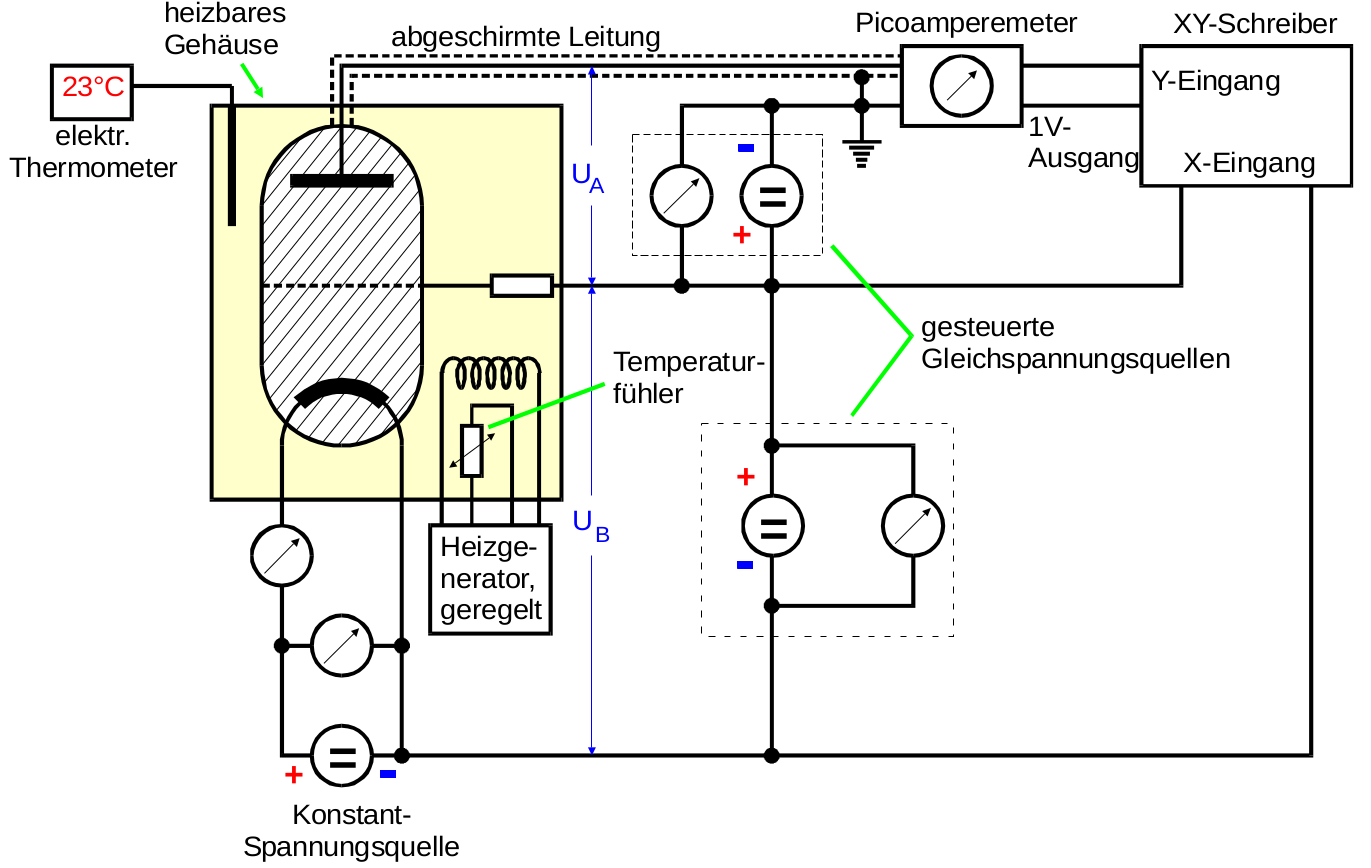
\includegraphics[width=\linewidth-70pt,height=\textheight-70pt,keepaspectratio]{content/Frankpraxis.png}
 \label{fig:frankpraxis}
\end{figure}

Zur Bestimmung der Energiedifferenz zwischen $E_1$ und $E_0$ sowie der Ionisierungsenergie
wird ein Aufbau nach Abb.\ref{fig:frankpraxis} verwendet. Den Kern bildet eine evakuierte Glasröhre,
in welcher sich ein Tropfen Quecksilber befindet. Über einen Heizgenerator lässt
sich das Quecksilber verdampfen , sowie dessen Sättigungsdampfdruck steuern. Die
Temperatur kann über ein digitales Thermometer abgelesen werden. Auf der einen Seite
der Glasröhre befindet sich eine Glühkathode, welche über eine Konstantspannungsquelle
versorgt wird. In der Mitte der Röhre befindet sich eine Beschleunigungselektrode,
am anderen Ende eine Auffängeranode. Zwischen Kathode und Beschleunigungselektrode
liegt die Beschleunigungsspannung $U_\text{B}$ an, zwischen Beschleunigungselektrode
und Aufängeranode eine Bremsspannung $U_\text{A}$. Beide werden jeweils über eine
eigene Gleichspannungsquelle versorgt. Der an der Auffängeranode ankommende Strom
wird mit einem Pikoamperemeter gemessen. Beide sind aufgrund der geringen Stromstärken
über eine abgeschirmte Leitung verbunden. Die auftretenden Kurven der Stromstärke in Abhängigkeit
von $U_\text{B}$ oder $U_\text{A}$ werden über einen XY-Schreiber grafisch dargestellt.
